\documentclass[UTF8]{ctexart}
\usepackage{amsmath}
\usepackage{amssymb}
\usepackage{background}
\usepackage{booktabs}
\usepackage{enumitem}
\usepackage{float}
\usepackage{fontspec}
\usepackage{geometry}
\usepackage{tasks}
\usepackage{tcolorbox}
\usepackage{xcolor}

\geometry{a5paper, top=0.1cm, left=1cm, right=1cm, bottom=1cm, footskip=0.1cm}
\setCJKmainfont[BoldFont={汉仪文黑-85W},ItalicFont={汉仪文黑-55W}]{汉仪文黑-55W}
\setfontfamily\Issue{Century Schoolbook}
\setfontfamily\Genshin{Genshin Teyvat Lingua Franca}
\newCJKfontfamily\TitleFont{思源宋体 CN Heavy}
\newfontfamily\timesnewroman{Times New Roman}

%————————————————可变部分——————————————————
\settasks{label={\Alph*.\ }, label-format={\color{cyan!50!black}}, item-format={\color{cyan!50!black}}}
\newcommand\col[1]{\textcolor{green!50!black}{#1}}
\newcommand\coll[1]{\textcolor{blue}{#1}}
\newcommand\dotting{\ .\ }
%——————————————————————————————————————————

%\pagestyle{fancy}
%\fancyhf{}
%\cfoot{\sffamily\footnotesize{-\ \thepage\ -}}
%\CTEXsetup[format = {\centering\bfseries\large}, beforeskip = 3pt, afterskip = 3pt]{section}

\colorlet{darkcyan}{cyan!50!black}
\newcommand\Black[1]{\textcolor[gray]{0.3}{#1}}
\newcommand\Brown[1]{\textcolor[HTML]{998A4E}{#1}}
\newcommand\Emph[1]{\colorbox{green!10}{\textcolor{green!30!black}{#1}}}
\newcommand\Notes[1]{\textcolor{yellow!50!black}{\small #1}}
\newcommand\Example[1]{\textcolor{cyan!70!black}{\small #1}}
\colorlet{note}{yellow!70!black}


\newcommand\IssueNumber{39}
\newcommand\Date{2024-10-31}
%\newcommand\Contributer{@金光日}
\newcommand\Subject{计算机网络}
\newcommand\Source{历年考研 408 真题}


\begin{document}
\backgroundsetup{contents=
\includegraphics{上半示例.png}, center, scale=1, angle=0, opacity=1}
\BgThispage
\begin{center}
%{\scriptsize\Issue \textcolor[HTML]{C8BA83}{\Genshin WEEKLY TIPS}}
\phantom{...}

{\Large\textcolor{brown!40!white}{\makebox[10cm][s]{\Genshin WEEKLY KNOWLEDGE TIPS}}}

\vspace{-2em}

{\Huge\bfseries\TitleFont \Black{知\ 识\ 小\ 料}}


\vspace{-0.1cm}
{\footnotesize \Brown{「电计 2203 班」周常规知识整理共享}}
\end{center}

\vspace{-0.5cm}


\begin{figure}[H]
\hspace{1cm}
\begin{minipage}[t]{0.3\textwidth}
\centering
    \Brown{\Genshin ISSUE}

    \vspace{-0.6cm}
    \Huge \Issue\slshape\bfseries\Black{\IssueNumber}
\end{minipage}
\hfill
\begin{minipage}[t]{0.35\textwidth}
\centering
    \Brown{日期:\Date} \\
%\vspace{-0.1cm}
%    \Brown{贡献者:\Contributer} \\
\vspace{-0.1cm}
    \Brown{学科:\Subject} \\
\vspace{-0.1cm}
    \Brown{来源:\Source}
\end{minipage}
\hspace{0.8cm}
\end{figure}

{\color{cyan!50!black}
《网络层·IP地址与 CIDR 子网专题》

\begin{description}
  \item[【简单挑战】] (2022)若某主机的 IP 地址是 183.80.72.48,子网掩码是 255.255.192.0,则该主机所在网络的网络地址是
  \begin{tasks}(2)
    \task 183.80.0.0
    \task 183.80.64.0
    \task 183.80.72.0
    \task 183.80.192.0
  \end{tasks}

  \item[【普通挑战】] (2018)某路由表中有转发接口相同的 4 条路由表项,其目的网络地址分别为 35.230.32.0/21、35.230.40.0/21、35.230.48.0/21 和 35.230.56.0/21,将该 4 条路由聚合后的目的网络地址为
  \begin{tasks}(2)
    \task 35.230.0.0/19
    \task 35.230.0.0/20
    \task 35.230.32.0/19
    \task 35.230.32.0/20
  \end{tasks}

  \item[【困难挑战】] (2019)若将 101.200.16.0/20 划分为 5 个子网,则可能的最小子网的可分配 IP 地址数是
  \begin{tasks}(4)
    \task 126
    \task 254
    \task 510
    \task 1022
  \end{tasks}

  \item[【无畏挑战】] (2021)现将一个 IP 网络划分为 3 个子网,若其中一个子网是 192.168.9.128/26,则下列网络中不可能是另外两个子网之一的是
  \begin{tasks}(2)
    \task 192.168.9.0/25
    \task 192.168.9.0/26
    \task 192.168.9.192/26
    \task 192.168.9.192/27
  \end{tasks}
\end{description}

}

\newpage
\backgroundsetup{contents=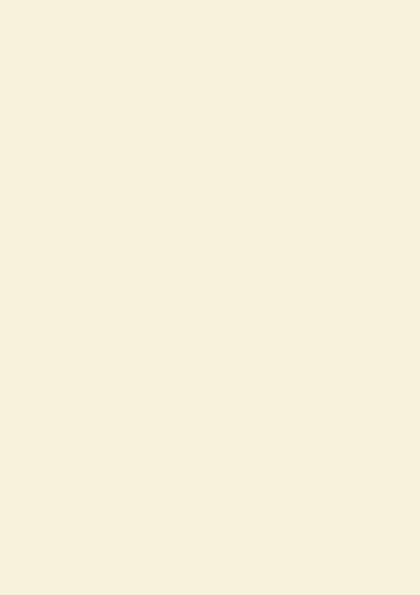
\includegraphics{空白示例.png}, center, scale=1, angle=0, opacity=1}
\BgThispage

\paragraph{【简单挑战】} 子网掩码中 1 的个数代表了IP地址中的子网部分,只需要用 IP 地址和子网掩码做\Emph{与运算}就可以得到网络地址。\textcolor{note}{(注:以下的例子中,IP 地址前两个数字不涉及,因此不展开为二进制。)}

\begin{table}[H]
    \centering
    \begin{tabular}{ccc@{\dotting}c@{\dotting}c@{\dotting}c}
         & IP 地址 & 183 & 80 & 01001000 & 00110000 \\
      \& & 子网掩码 & \col{255} & \col{255} & \col{11}000000 & 00000000 \\
    \hline
         & 网络地址 & \col{183} & \col{80} & \col{01}000000 & 00000000 \\
    \end{tabular}
\end{table}

得到的结果为:183.80.64.0,选 B。

\paragraph{【普通挑战】} 四条路由表项的目的网络地址都是 21 位网络号(\col{绿色}文字所示,下同),展开如下:

\begin{table}[H]
    \centering
    \begin{tabular}{c@{\dotting}c@{\dotting}c@{\dotting}c}
        \col{35} & \col{230} & \col{00100}000 & 00000000 \\
        \col{35} & \col{230} & \col{00101}000 & 00000000 \\
        \col{35} & \col{230} & \col{00110}000 & 00000000 \\
        \col{35} & \col{230} & \col{00111}000 & 00000000 \\
    \end{tabular}
\end{table}

路由聚合是一种把若干个 IP 地址合并为一个更大的地址块的方法,关键在于\Emph{取公共前缀}。

这四个地址的第三段中,前三位都是相同的 \col{001},因此取公共前缀,这三位是能够聚合的最大位数。总共的网络部分有 $16+3=19$ 位:

\begin{table}[H]
    \centering
    \begin{tabular}{c@{\dotting}c@{\dotting}c@{\dotting}c}
        \col{35} & \col{230} & \col{001}00000 & 00000000 \\
    \end{tabular}
\end{table}

因此为 35.230.32.0/19,选 C。

\paragraph{【困难挑战】} 将 101.200.16.0/20 拆成二进制如下:

\begin{table}[H]
    \centering
    \begin{tabular}{c@{\dotting}c@{\dotting}c@{\dotting}c}
        \col{101} & \col{200} & \col{0001}0000 & 00000000 \\
    \end{tabular}
\end{table}

如果想要划分为 5 个子网,一个直观的想法是\Emph{平均分配}。由于 5 个子网可以用 3 位二进制数($000\sim 100$)表示,借用原主机号的前 3 位用来组成新的子网,是一种办法。此时,网络号有 $20+3=23$ 位,主机号有 $32-23=9$ 位,有 $2^9-2=510$ 个 IP 地址可以分配。

但,这是可能的\Emph{最小}子网吗?

考虑借用《计算机组成原理》课的指令系统「扩展操作码」的思想,不平均分配,而是让主机数\Emph{越分越小},像这样:

\begin{table}[H]
    \centering
    \begin{tabular}{c@{\dotting}c@{\dotting}c@{\dotting}c}
        \col{101} & \col{200} & \col{0001}\coll{0}xxx & xxxxxxxx \\
        \col{101} & \col{200} & \col{0001}\coll{10}xx & xxxxxxxx \\
        \col{101} & \col{200} & \col{0001}\coll{110}x & xxxxxxxx \\
        \col{101} & \col{200} & \col{0001}\coll{1110} & xxxxxxxx \\
        \col{101} & \col{200} & \col{0001}\coll{1111} & xxxxxxxx \\
    \end{tabular}
\end{table}

\begin{itemize}
    \item 对于第一子网,将第 21 位的 \coll{0} 作为新的网络号,余下为主机号;
    \item 对于第二子网,将第 21 位的 \coll{1} 作为「扩展码标志」,第 22 位的 \coll{0} 作为新的网络号,余下为主机号;
    \item 对于第三、第四子网,依次类推。此时到 $21\sim 24$ 位的 \coll{1110} 都是网络号;
    \item 对于第五子网,为了保证子网覆盖全部 IP 地址空间,不取新的网络号,而是将 24 位改成 \coll{1} 作为网络号。
\end{itemize}

此时,最小的子网为第四、第五子网,有 24 位网络号,8 位主机号。除去主机号为全零和全一的 2 种情况,因此可分配的 IP 地址有 $2^8-2=254$ 个。选 B。

\paragraph{【无畏挑战】} 按照惯例,先把题干和选项的 IP 地址展开:

\begin{table}[H]
    \centering
    \begin{tabular}{cc@{\dotting}c@{\dotting}c@{\dotting}c}
        题干 & \col{192} & \col{168} & \col{00001001} & \col{10}000000 \\
        A.   & \col{192} & \col{168} & \col{00001001} & \col{0}0000000 \\
        B.   & \col{192} & \col{168} & \col{00001001} & \col{00}000000 \\
        C.   & \col{192} & \col{168} & \col{00001001} & \col{11}000000 \\
        D.   & \col{192} & \col{168} & \col{00001001} & \col{110}00000 \\
    \end{tabular}
\end{table}

划分子网的原则是,要求子网之间的 IP 地址不重叠,且覆盖全部的 IP 地址空间。由于我们不知道原网络的 IP 地址,所以这题采用选项代入法:若取题干和待取选项作为两个 IP 子网,能否找到剩下的\Emph{唯一的}子网。不能找到的即为本题答案。

\begin{table}[H]
    \centering
    \begin{tabular}{cc@{\dotting}c@{\dotting}c@{\dotting}c}
        题干 & \col{192} & \col{168} & \col{00001001} & \col{10}xxxxxx \\
        A.   & \col{192} & \col{168} & \col{00001001} & \col{0}xxxxxxx \\
        剩下的子网 &  \col{192} & \col{168} & \col{00001001} & \col{11}xxxxxx \\
    \end{tabular}
\end{table}

\begin{table}[H]
    \centering
    \begin{tabular}{cc@{\dotting}c@{\dotting}c@{\dotting}c}
        题干 & \col{192} & \col{168} & \col{00001001} & \col{10}xxxxxx \\
        C.   & \col{192} & \col{168} & \col{00001001} & \col{11}xxxxxx \\
        剩下的子网 &  \col{192} & \col{168} & \col{00001001} & \col{0}xxxxxxx \\
    \end{tabular}
\end{table}

\begin{table}[H]
    \centering
    \begin{tabular}{cc@{\dotting}c@{\dotting}c@{\dotting}c}
        题干 & \col{192} & \col{168} & \col{00001001} & \col{10}xxxxxx \\
        D.   & \col{192} & \col{168} & \col{00001001} & \col{110}xxxxx \\
        剩下的子网 &  \col{192} & \col{168} & \col{00001001} & \col{111}xxxxx \\
    \end{tabular}
\end{table}

从上面的推导可以看出,选择 A,C,D 都可以找到剩下的\Emph{唯一的}子网。但是如果用 B 来试试,就会这样:

\begin{table}[H]
    \centering
    \begin{tabular}{cc@{\dotting}c@{\dotting}c@{\dotting}c}
        题干 & \col{192} & \col{168} & \col{00001001} & \col{10}xxxxxx \\
        B.   & \col{192} & \col{168} & \col{00001001} & \col{00}xxxxxx \\
        剩下的子网-1 &  \col{192} & \col{168} & \col{00001001} & \col{01}xxxxxx \\
        剩下的子网-2 &  \col{192} & \col{168} & \col{00001001} & \col{11}xxxxxx \\
    \end{tabular}
\end{table}

如果选择题干与 B,则按照划分子网原则,剩下的子网必须要 2 个才得以覆盖全部 IP 地址空间。因此,在题干所述的 3 个子网中,B 选项不能做除题干外的两个子网之一。因此选 B。

\backgroundsetup{contents=
\includegraphics{下半示例.png}, center, scale=1, angle=0, opacity=1}
\BgThispage
\vspace{1em}
{\color{cyan!80!black}
【结论】BCBB

【点评】这是四道计网的考研题,由易到难,涉及网络层的 IP 地址、CIDR(无分类域间路由选择)的相关知识。解决这类问题的关键,在于正确地区分开网络部分和主机部分。
}


\end{document} 